\documentclass{beamer}
%\documentclass[handout]{beamer}


%LaTeXAccusativusEnkelvoud maakt LaTeGeM door \Tex aan te passen naar TeGeM en daarna terug te zetten naar oorspronkelijke TeX
\newcommand{\oudeTeX}{\TeX}
\newcommand{\LaTeXAccusativusEnkelvoud}{\renewcommand{\TeX}{\makeatletter T\kern -.1667em\lower .5ex\hbox {E}\kern -.125emG\@\hspace{-0.1ex}\raisebox{0.50ex}{{\scriptsize E}}\hspace{-0.1ex}M\makeatother }\LaTeX	\renewcommand{\TeX}{\oudeTeX}}
%\makeatletter T\kern -.1667em\lower .5ex\hbox {E}\kern -.125emX\@\makeatother}

\title{\LaTeX-cursus 2021\\
Week 2: Essentieel}
\author{\TeX niCie}
\date{4 oktober 2021}


\usepackage[dutch]{babel}
\selectlanguage{dutch}
\usepackage{marvosym,cursus,hyperref,calc,verbatim,mathrsfs,graphicx}
%yfonts
\newcommand\metcode[3]{%
\begin{columns}
\column{#1\textwidth}
#2
\column{\textwidth-#1\textwidth}
#3
\end{columns}%
}

% Hierdoor staat er Voorbeeld in plaats van example boven exampleblocks.
\let\trans\translate
\renewcommand\translate[1]{\ifthenelse{\equal{#1}{Example}}{Voorbeeld}{\trans{#1}}}


\usetheme{aes2}
%\usetheme{Frankfurt} %Een ander thema als je deze niet wil gebruiken
%\usecolortheme{dolphin} %crane of dolphin
%\useinnertheme{circles}
%\useoutertheme{smoothbars}

%\setbeamercovered{dynamic}

\begin{document}


\begin{frame}
\titlepage
\end{frame}



\section*{Introductie}


\begin{frame}
\frametitle{Vorige week}
Vorige week hebben we het volgende gedaan:
\begin{itemize}
\item Opzet \LaTeX{} vs. Word
\item Formules in \LaTeX{} en de symbolen die je daarin kan gebruiken
\item Het oplijnen van formules en matrices
\item Plaatjes invoegen (zonder onderschrift)
\end{itemize}
\end{frame}


\begin{frame}
\frametitle{Deze week}
\begin{itemize}
	\item Opmaak van je document en tekst (kopjes, header, footer, kantlijnen,...)
	\item Plaatjes en andere niet-tekst elementen met onderschrift
	\item Verwijzen binnen je document en een automatische inhoudsopgave
	\item Lijsten maken zoals deze lijst eruitziet
	\item Een stelling
\end{itemize}
\end{frame}

\begin{frame}{SLIDES ZIJN BESCHIKBAAR}
	\huge{Zie hiervoor onze website: \url{www.a-eskwadraat.nl/latex}}
\end{frame}

\section{Opmaak}
\begin{frame}
\frametitle{Verschil in opmaak}
	\begin{tabular}{c c}
		\fbox{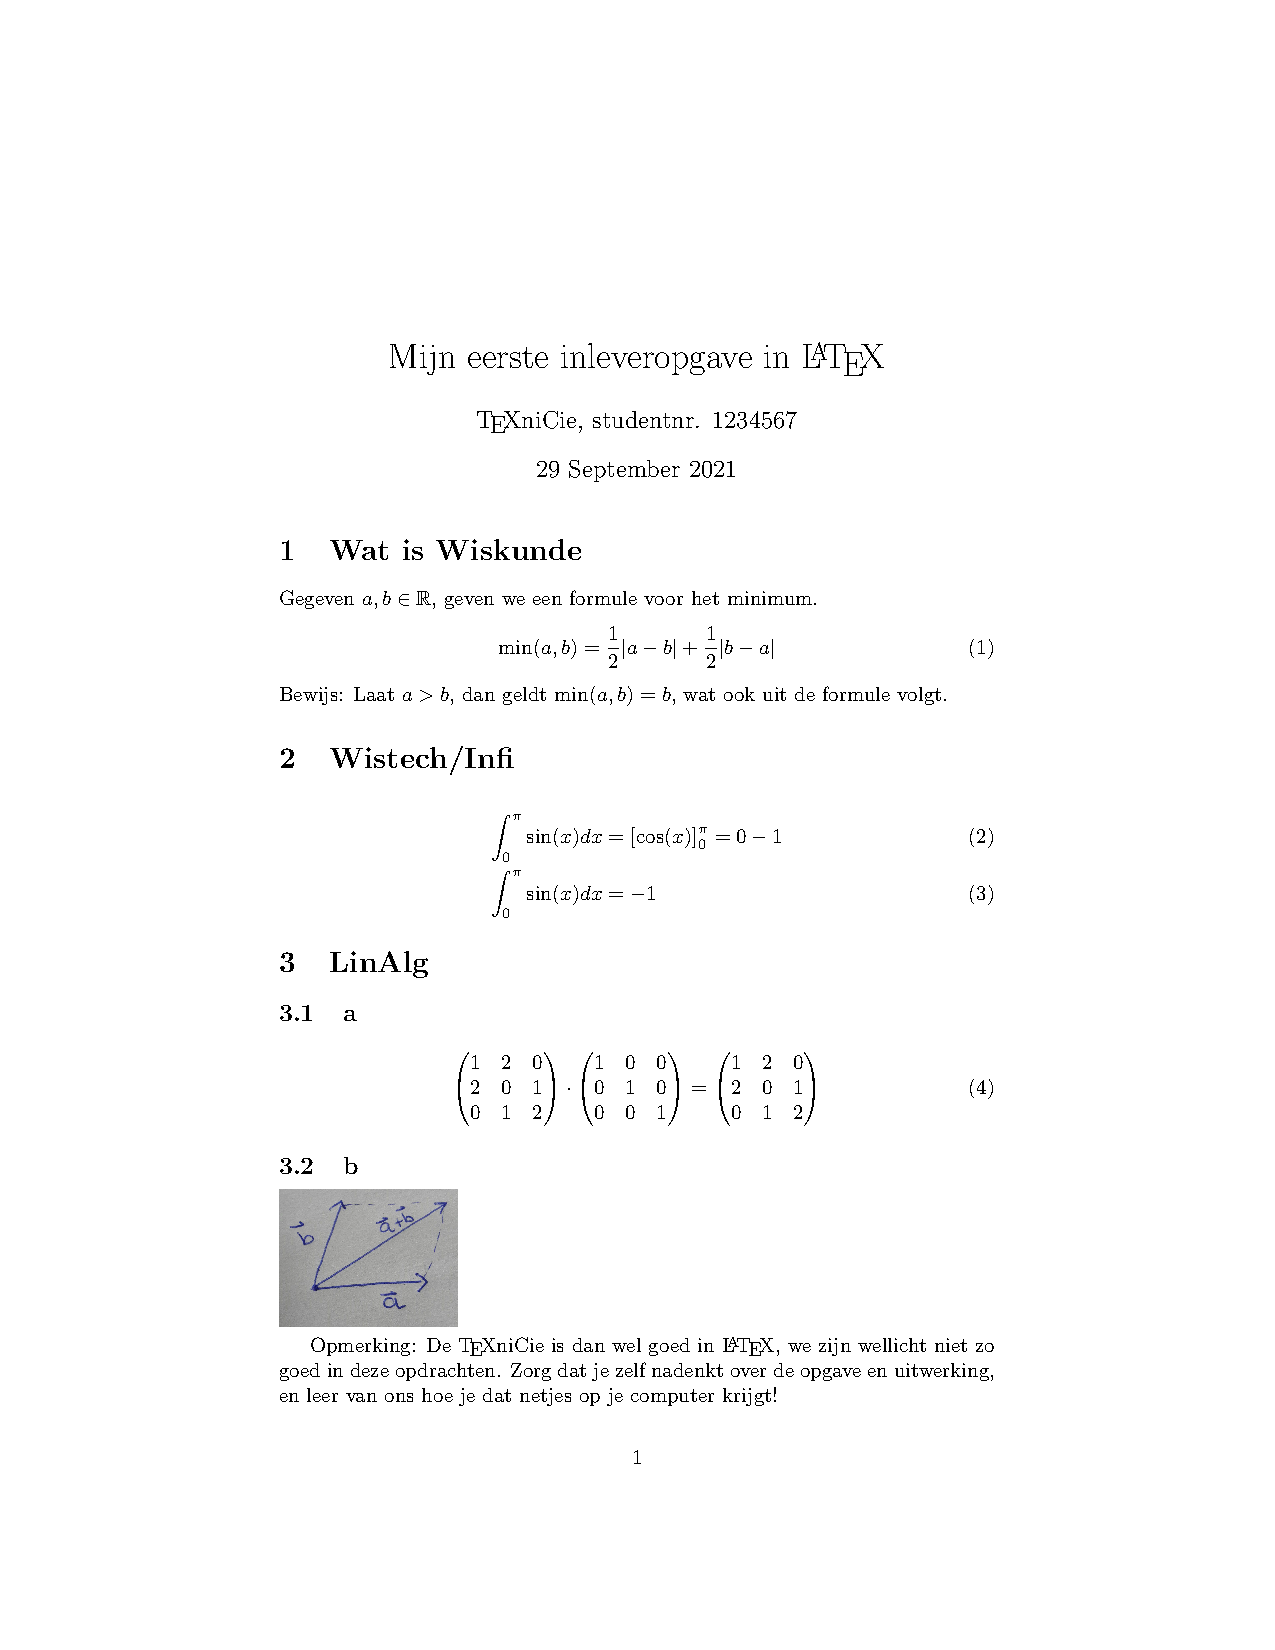
\includegraphics[width=0.4\textwidth]{assets/voorbeeldweek1.pdf}}
		& \fbox{\includegraphics[width=0.4\textwidth, page=2]{assets/voorbeeldweek2.pdf}}
	\end{tabular}
\end{frame}

\begin{frame}
	\frametitle{Wat we voor mogelijkheden zien:}
	\begin{itemize}
		\item Een header, inclusief links en rechts uitlijning
		\item Minder witruimte links en rechts op de pagina
		\item Lijsten in deel 1
		\item Plaatje met onderschrift
		\item Een footer met uitlijning en pagina zoveel van totaal
		\item (Misschien is je in de andere pagina's van het voorbeeld al meer opgevallen)
		\item Er is veel meer mogelijk, afhankelijk van je smaak en hoeveel werk je erin wil steken...
	\end{itemize}
\end{frame}

\begin{frame}
	\frametitle{Uitlijning en pagina-layout}
	Voor de paginamarges: \texttt{\textbackslash usepackage\{geometry\} }\\
	Optioneel kan je echt alle dimensies van je document meegeven:
	\begin{figure}
			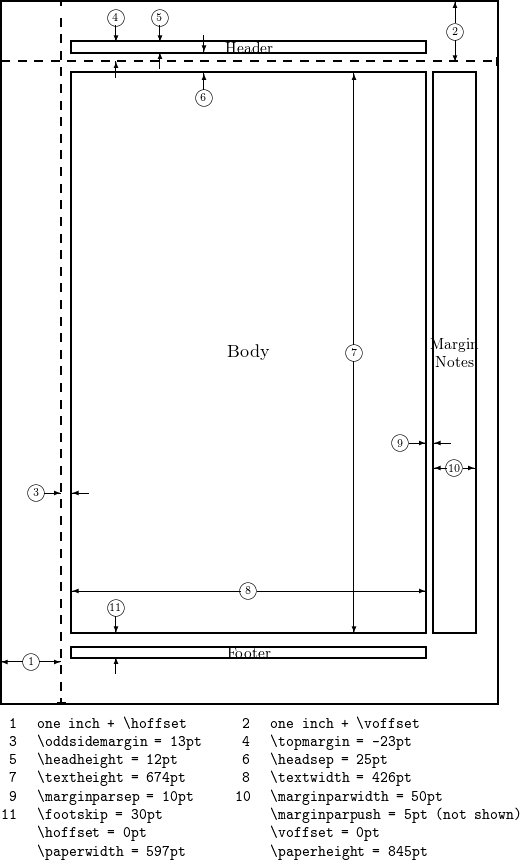
\includegraphics[height=0.9\textheight]{assets/Layout-dimensions.png}
			%\caption{Zoals je kan zien in dit plaatje op de site van Overleaf.}
	\end{figure}
\end{frame}

\begin{frame}
	\frametitle{Headers en footers}
	Wellicht wil je op elke pagina van je inleveropgave iets neerzetten, zoals in het voorbeeld. De titelpagina heeft standaard een andere opmaak, zonder header en footer! Wat het wordt definieer je in de preamble:
	\begin{block}{Code}
		\texttt{\textbackslash usepackage\{fancyhdf\}}\\
		\texttt{\textbackslash pagestyle\{fancy\}}\\
		\texttt{\textbackslash fancyhf\{ \}}\\
		\texttt{\textbackslash rhead\{{\textnormal{Hier wat je rechts in je header uitgelijnd wil}}\}}\\
		\texttt{\textbackslash lhead\{{\textnormal{Hier wat je links in je header uitgelijnd wil}}\}}\\
		\texttt{\textbackslash rfoot\{{\textnormal{Hier wat je rechts in je footer uitgelijnd wil}}\}}\\
		\texttt{\textbackslash lfoot\{{\textnormal{Hier wat je links in je footer uitgelijnd wil}}\}}
	\end{block}
\end{frame}

\begin{frame}
	\frametitle{Andere handige layout codes}
	Voor het horizontaal opvullen/leeglaten van je (tekst)regel, minus wat je nog aan de rechterkant wil zetten kan je \texttt{\textbackslash hfill} gebruiken:\\
	Links \hfill Rechts\\
	
	Voor het verticaal opvullen/leeglaten van je pagina, \vfill minus wat je nog onderaan wil zetten gebruik je \texttt{\textbackslash vfill}.
\end{frame}

\begin{frame}
	\frametitle{Oefening: maak de layout van voorbeeld van deze week}
	Probeer de opmaakelementen (dus niet de inhoudsopgave, deel 1, 2.1,  2.2 en de wiskunde van deel 3) na te maken in een nieuw document. \begin{block}{code}
	\texttt{\textbackslash usepackage\{fancyhdf, lastpage\}}\\
	\texttt{\textbackslash pagestyle\{fancy\}}\\
	\texttt{\textbackslash fancyhf\{ \}}\\
	\texttt{\textbackslash rhead\{{\textnormal{Hier wat je rechts in je header uitgelijnd wil}}\}}\\
	\texttt{\textbackslash lhead\{{\textnormal{Hier wat je links in je header uitgelijnd wil}}\}}\\
	\texttt{\textbackslash rfoot\{Pagina \textbackslash thepage \textbackslash text\{van \textbackslash pageref\{LastPage\}\}\} }
	\end{block}
	Klaar? Bekijk de extra oefeningen van vorige week over tekstkleuren en grootes op \url{https://www.vkuhlmann.com/latex/exercises/2021-09-Cursus/week1}\\
	Weer klaar? Probeer de wiskunde van deel 3 toe te voegen. %(zoek symbolen op in de presentatie van vorige week of teken ze in \url{detexify.kirelabs.org/}).
	
\end{frame}

\section{Figuren en tabellen}
\begin{frame}
	\frametitle{Figuren}
	\begin{block}{code opzet}
		\texttt{\textbackslash begin\{figure\}[Plaatsbepaler]\\
			\textbackslash centering\\
			\textbackslash includegraphics[optionals]\{plaatje.png\}\\
			\textbackslash caption\{Onderschrift\}
			\textbackslash label\{fig:plaatje\}
		\textbackslash end\{figure\}}
	\end{block}
	\begin{block}{output}
	{\begin{figure}
	\centering
	%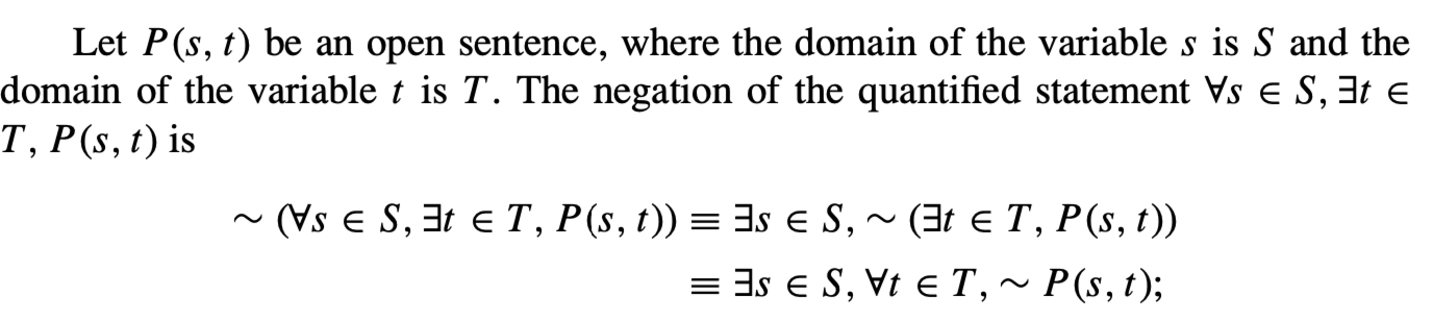
\includegraphics{plaatje.png}
    \includegraphics[height=2cm]{example-image-a}
	\caption{Onderschrift}
	\label{fig:plaatje}
	\end{figure}}
	\end{block}
\end{frame}
\begin{frame}{Meerdere plaatjes in \'e\'en figuur omgeving}
	\texttt{\textbackslash begin\{figure\}\\
		\quad	\textbackslash begin\{subfigure\}[plaatsing]\{Breedte\}\\
			\qquad	\textbackslash centering\\
			\qquad	\textbackslash includegraphics...\\
			\qquad	\textbackslash caption\{onderschrift subfig a\}\\
			\qquad	\textbackslash label\{fig:subfiga\}\\
		\quad	\textbackslash end\{subfigure\}\\
		\quad	... code herhalen voor meer subfiguren ...\\
		\quad	\textbackslash caption\{onderschrift voor alle plaatjes bijelkaar\}\\
		\quad	\textbackslash label\{fig:subfigsabcde\}\\
		\textbackslash end\{figure\}
	}
\end{frame}
\begin{frame}
	\frametitle{Tabellen}
	\begin{block}{code opzet}
		\texttt{\textbackslash begin\{table\}[Plaatsbepaler]\\
		\quad	\textbackslash centering\\
		\quad	\textbackslash begin\{tabular\}\{LAYOUT\}\}\\
		\qquad	Rij1 \& \$wiskunde\$ \& tekst \textbackslash \textbackslash\\
		\qquad	Nieuwe regel \& met net zoveel \& als kolommen in\\
		\qquad de hele tabel\textbackslash
			\textbackslash\\
		\qquad	\textbackslash hline\\
		\qquad	Laatste \& regel \& tabel\\
		\quad	\textbackslash end\{tabular\}\\
		\quad	\textbackslash caption\{Onderschrift\}\\
		\quad	\textbackslash label\{tab:tabel\}\\
			\textbackslash end\{table\}}
	\end{block}
\end{frame}
\begin{frame}
	\frametitle{Tabellen}
	Layout voor elke rij:
	\begin{itemize}
		\item \texttt{l,c,r} voor uitlijning van elementen, net zoveel letters als kolommen
		\item je kan verticale lijnen maken door $|$ te plaatsen tussen de letters (dubbele lijnen door $||$)
	\end{itemize}
Kies bijvoorbeeld \texttt{||r|c|l||}, dan ziet de tabel er zo uit:
	\begin{block}{output}
		{\begin{table}
				\centering
				\begin{tabular}{||r|c|l||}
					Rij1 & $wiskunde$ & tekst\\
					Nieuwe regel & met net zoveel & als kolommen in de hele tabel\\
					\hline
					Laatste & regel & tabel
				\end{tabular}
				\caption{Onderschrift}
				\label{tab: tabel}
		\end{table}}
	\end{block}
\end{frame}

\begin{frame}[allowframebreaks]{De plaatsbepaler}
		De plaatsbepaler is een argument [in deze recht haken dus] dat aangeeft waar je precies het figuur/de tabel hebben wilt. Deze precies is niet zo precies als je bij Word kan aangeven, waarschijnlijk krijg je er ooit ruzie mee dus we gaan ook wat oplossingen na.
	
	\framebreak
	Je kunt gebruik maken van de volgende plaatsbepalers:
	
	\begin{table}
		\center
		\begin{tabular}{lll}
			h &	here    & Plaats het figuur \alert{ONGEVEER} hier in de tekst. \\
			t & top     & Plaats het figuur bovenaan de bladzijde.\\
			b & bottom  & Plaats het figuur onderaan de tekst. \\
			p &	page    & Plaats het figuur op een speciale pagina voor figuren. \\
			! &	        & Dit commando kun je achter \'e\'en van de bovenstaande  \\ 
			&         & plakken en overreed de interne parameters voor het\\
			&         & vinden van een goede positie.\\
			H & HERE    & Plaats het figuur precies \alert{HIER} in het document.\\
			&         & Dit lijkt veel op het h! commando.
		\end{tabular}
	\end{table}
	\framebreak
	
	Het maakt niet uit in welke volgorde h, p, t, b of ! staan, \LaTeX{} gebruikt de volgende volgorde: 
	\begin{itemize}
		\item Eerst kijkt het of er een h tussen staat. Als er een h is opgegeven, probeert \LaTeX{} meteen het figuur te plaatsen.
		\item Als dat niet gelukt is en er staat een t, probeert het het plaatje bovenaan te plaatsen.
		\item Daarna probeert \LaTeX{} een b.
		\item Als het plaatje nog steeds niet past, stopt \LaTeX{} het plaatje in de wachtrij. Deze wordt geleegd, als er een nieuwe pagina wordt aangemaakt.
	\end{itemize}
	\framebreak
	
	Veel gebruikte oplossingen om het plaatje toch te krijgen waar jij wil:
	\begin{itemize}
		\item Maak het plaatje kleiner zodat er minder problemen zijn
		\item Verplaats de code voor een plaatje iets naar voren om het plaatje wel op de juiste plek te krijgen
		\item Eindig je pagina na de tekst waarna je het plaatje wil en gebruik \texttt{\textbackslash clearpage} Zolang de rest van de pagina groot genoeg is voor het plaatje komt het plaatje onderaan.
		\item Kies ervoor alleen te refereren naar plaatjes in je tekst en alle plaatjes op een aparte pagina te zetten.
	\end{itemize}
We gaan eerst wat oefenen, voor we overgaan op de referenties.
\end{frame}

\begin{frame}
	\frametitle{Oefenen met figuren en tabellen}
	Vul in je eerder gemaakte document sectie twee in met een leuk plaatje (mag ook iets anders zijn) en de gegeven tabel. Schrijf eerst nog letterlijk de captions over, straks kan je die in de tabel vervangen door een referentie. \\
	Klaar?	Voeg aan het eind van sectie 2 een plaatje toe (bijvoorbeeld van je favoriete dier), die precies geplaatst wordt tussen de tabel en de titel van sectie 3. Kijk ook of het je lukt hem helemaal bovenaan of onderaan de pagina te krijgen.
\end{frame}
	
\section{Verwijzingen}
\begin{frame}[allowframebreaks]
	\frametitle{Verwijzen}
	Stel je wil een extra plaatje op de voorpagina, dan wordt figuur 1 (in sectie 2) hernoemt naar figuur 2, het is immers nu het tweede figuur wat we plaatsen, maar nu staat er in het onderschrift van de tabel nog figuur 1!
	
	\LaTeX{} kan automatisch refereren naar het juiste nummer, zonder dat jij je zorgen hoeft te maken welk nummer die precies heeft gekregen. Sterker nog, dat kan ook met de \texttt{align} en \texttt{equation} omgevingen als je naar formules wil refereren. Handig als je een paar regels later een vorige formule wil gebruiken. Je kan ook naar secties en subsecties verwijzen.
	
	\framebreak
	
	Om te kunnen verwijzen moet je dingen een naampje geven. Dit doe je door het commando \alert{\texttt{\textbackslash label\{fig:tekening\}}}. De conventie is om de eerste twee of drie letters te verwijzen naar wat voor soort iets het is, daarna een : om vervolgens een korte tekst te geven als omschrijving voor jezelf
	
	\begin{table}
		\centering
		\begin{tabular}{c|l}
			eq:&	equation \\ 
			fig:&	figure \\
			tab:&	table \\
			chap: &	chapter \\
			sec:&	section \\
			subsec:&	subsection \\
			itm:&	enumerated list item \\
			app:&	appendix subsection
		\end{tabular}
	\end{table}

	\framebreak
	Vervolgens refereer je terug aan je label door een commando. Er zijn verschillende gevallen:
	\begin{description}
		\item[handmatig:] Je kan zelf schrijven: \texttt{Zie Figuur \textbackslash ref\{fig:tekening\}}.
		\item[automatisch] Het commando \texttt{\textbackslash autoref\{fig:tekening\}} geeft als output \textit{Figuur 4}. 
		\item[pagina]  Het commando \texttt{\textbackslash pageref} verwijst naar de pagina waarop iets is geplaatst (of begint als het langer is dan een pagina).
		\item[formule] gebruik \texttt{vergelijking \textbackslash eqref\{eq:vergelijking\}} voor \textit{vergelijking (3)}.
	\end{description}
\end{frame}
	
\begin{frame}
	\frametitle{Taal}
	Pas hierbij op dat je de juiste taal gebruikt in \LaTeX, dat is het Babel package. Standaard staat die in het Engels en zullen je figuren dus \textit{Figure 4} heten en autorefereren naar \textit{Figuur 4}. Zet in je preamble \texttt{\textbackslash usepackage[dutch]\{babel\}} om dit te veranderen naar Nederlandse namen.
\end{frame}	

\begin{frame}{Inhoudsopgave}
	Een inhoudsopgave is nog gemakkelijker dan \texttt{\textbackslash maketitle}, waar je nog de titel, auteur en datum op moet geven. \LaTeX{} houdt namelijk automatisch je secties bij. Je print de inhoudsopgave met \texttt{\textbackslash tableofcontents}.
	Dit gebeurt wel alleen bij secties die een nummer hebben.
	Iets wat niet automatisch in de inhoudsopgave komt handmatig toevoegen kan door\\ \texttt{\textbackslash addto contentsline\{toc\}\{section\}\{Naam\}},\\ waar \texttt{toc} staat voor Table Of Contents, \texttt{section} voor welk soort element en de laatste entry de naam is die verschijnt in de inhoudsopgave.
\end{frame}

\begin{frame}{oefenen}
	Vul je document aan met de referenties en inhoudsopgave. Probeer verschillende manieren en plekken om labels te plaatsen. Let vooral op de plaatsing van \texttt{\textbackslash caption} en \texttt{\textbackslash label} bij je plaatje!\\
	Klaar? Neem een koekje!
\end{frame}

\section{Lijsten}
\begin{frame}{Itemize, enumerate}
	\begin{itemize}
		\item de itemize-omgeving geeft dit als output.
		\item gebruik code: \texttt{\textbackslash begin\{itemize\} \dots \textbackslash end\{itemize\}}
		\item tussendoor gebruik je bij elk deel van de tekst \texttt{\textbackslash item}
		\item \texttt{\textbackslash item Het volgende punt wordt dus zo}
		\item Het volgende punt wordt dus zo
	\end{itemize}
In plaats van itemize kan je ook \texttt{enumerate} gebruiken voor getallen. Je kan op elk moment een item laten nummeren met $n$ door voor het nieuwe item in de code het commando \texttt{\textbackslash setcounter{enumi}\{$n-1$\}} zetten (volgende week meer over die counters).
\end{frame}

\begin{frame}{Description}
	Je kan ook een lijst maken die je een woord meegeeft ipv dat er een getal of punt staat, dat is de \texttt{description} omgeving. Het woord geef je op de volgende manier mee:\\
	\texttt{\textbackslash item[omschrijving]}.
\end{frame}

\begin{frame}{oefenen}
	Vul sectie 1 in je document op zoals in het voorbeelddocument van deze week.
\end{frame}

\section{Stellingen en bewijzen}
\begin{frame}[allowframebreaks]{Stellingen en bewijzen}
	Voor de wiskundestudenten is er ook een speciale omgeving zodat stellingen en bewijzen er netjes uitzien.
	Dit is de theorem omgeving uit het package \texttt{amsmath}.
	In je preamble kan je aangeven wat voor soort omgevingen je wil maken.
	\texttt{\textbackslash newtheorem\{stelling\}\{Stelling\}}\\
	\framebreak
	Op deze manier kan je bijvoorbeeld netjes stellen:
	\begin{block}{code}
		\texttt{\textbackslash begin\{stelling\}[Mijn eerste stelling]\\
			Laat \$a>b\$, dan \$a-b>0\$.\\
			\textbackslash end\{stelling\}\\
			\textbackslash begin\{proof\}\\
				Haal \$b\$ af van beide kanten van het ongelijkheidsteken, dit verandert niet de richting van het ongelijkheidsteken.\\
			\textbackslash end\{proof\}}
	\end{block}
\end{frame}

\begin{frame}{oefenen}
	Voeg de stelling van de vorige slide toe aan een vierde pagina van je document. Zorg dat, waar dat nog niet zo is, de rest van je document vergelijkbaar is met het voorbeelddocument van week 2.
	\vfill
	NB: zowel deze slides als dat voorbeeld staan op onze site: \url{www.a-eskwadraat.nl/latex}!
\end{frame}

\end{document}
